% HaluRISC Course Paper — modular entry point
%
% Structure: paper.tex only holds the preamble and \input{}s the numbered
% modules below (add/remove modules by editing this file — never content here).
%
%   report/
%   ├── paper.tex            <- main entry point (this file)
%   ├── 0.1.title.tex        <- title page
%   ├── 0.2.abstract.tex     <- abstract
%   ├── 1.intro.tex
%   ├── 2.related_work.tex
%   ├── 3.method.tex
%   ├── 4.experiments.tex
%   ├── 5.web_application.tex
%   ├── 6.results_discussion.tex
%   ├── 7.conclusion.tex
%   ├── 8.reproducibility.tex
%   ├── 9.ethics.tex
%   └── ref.bib             <- BibTeX references
%
% Compile (run twice for references):
%   pdflatex paper.tex && bibtex paper && pdflatex paper.tex && pdflatex paper.tex
%   (or: latexmk -pdf paper.tex)
%
% Figures: ../artifacts/figures/*.pdf, ./screenshots/*.png
\documentclass[12pt,a4paper]{article}

\usepackage[T1]{fontenc}
\usepackage[utf8]{inputenc}
\usepackage[a4paper,margin=0.75in]{geometry}
\usepackage{graphicx}
\usepackage{booktabs}
\usepackage{array}
\usepackage{parskip}
\usepackage{enumitem}
\usepackage{caption}
\usepackage{tikz}
\usepackage{amsmath}

\setlength{\parskip}{0.35em}
\setlist{topsep=2pt, itemsep=1pt, parsep=1pt}
\emergencystretch=2em
\sloppy
\captionsetup{font=small,labelfont=bf}

\graphicspath{{../artifacts/figures/}{./figures/}{./screenshots/}}

% University logo (renders only if an image file is present)
\newif\ifuiu
\IfFileExists{./uiu.png}{\uiutrue}{}
\IfFileExists{./uiu.jpg}{\uiutrue}{}
\IfFileExists{./uiu.pdf}{\uiutrue}{}

\begin{document}

% Title page — keep names/affiliations up to date here.
\begin{titlepage}
    \centering

    \begin{center}
        \ifuiu
            
\includegraphics[scale=0.22]{./uiu}
        \else
            \textbf{[Place UIU logo as uiu.png/jpg/pdf in the report folder]}
        \fi
    \end{center}

    {\scshape United International University}\\[0.3em]
    {\scshape Department of Computer Science and Engineering}

    \vspace{2cm}

    {\scshape Journal-Style Term Paper}

    \vspace{1.2cm}

    {\Large\bfseries HaluRISC: A Calibrated and Explainable Machine Learning\\[0.2em]
    Framework for Hallucination Risk Prediction in Black-Box LLM Outputs}

    \vspace{1.2cm}

    \vfill

    { Submitted By}

    \vspace{0.5cm}

    \begin{tabular}{lc}
        \bfseries Md. Atikur Rahaman & 0112310298 \\
        \bfseries Saiful Alam Sabbir & 0112320105 \\
        \bfseries MD. Miraz Ahamed   & 0112310524 \\
    \end{tabular}

    \vfill

    { Supervision}

    \vspace{0.4cm}

    {\bfseries Ohidujjaman Tuhin, PhD}\\
    Associate Professor, Dept. of Computer Science and Engineering\\
    United International University

    \vspace{0.6em}

    Course: Machine Learning, Section: E

    \vfill

    \the\year

\end{titlepage}

\newpage

% Abstract — Version B numbers, frozen at commit 9bdb329e (manifest.frozen.json).
\begin{abstract}
\noindent
Large language models produce fluent output that is occasionally fabricated, and detecting these hallucinations is expensive, opaque, or requires access to model internals in most existing approaches. This paper presents HaluRISC, a lightweight black-box framework that predicts hallucination risk from the question, a reference context, and the candidate answer. The system builds 26 engineered evidence-consistency features across seven groups, covering lexical overlap, named entities, NLI entailment, numeric consistency, hedging, semantic similarity, and length, then feeds them to a tuned XGBoost classifier with calibrated probabilities and SHAP explanations. On the HaluEval QA benchmark (20{,}000 rows, 70/15/15 stratified split), the calibrated model reaches F1 = 0.9846, AUROC = 0.9979, and MCC = 0.9697, with an expected calibration error of 0.0045 before any recalibration. A small-sample recalibration on natural RAGTruth responses cuts the ECE on that corpus from 0.8185 to 0.1335, which shows the value of re-calibrating for the target domain. Zero-shot transfer to natural RAGTruth QA still fails (F1 = 0.3022), an honest limitation the paper discusses in detail. The full analysis runs in about 62~ms per sample on a CPU and costs roughly 100 times less than an LLM-as-judge baseline while reaching a higher F1 on a measured 200-sample set. The complete system is deployed as a FastAPI backend with a Next.js and assistant-ui web dashboard for live demonstration.
\end{abstract}


% Chapter 1 — Introduction.
\section{Introduction}

Large language models are increasingly embedded in real products---chatbots, retrieval-augmented question answering, and content-review tools---where a confidently wrong answer has a real cost. LLMs occasionally generate text that is fluent but factually unsupported, an effect known as \emph{hallucination}. Detecting hallucinations is therefore a first-class safety problem.

The dominant detection strategy asks a strong LLM to judge its own output (SelfCheckGPT \cite{selfcheck}) or to act as an external judge. Such approaches are slow (seconds per response), expensive at scale (API fees per call), and opaque (no feature-level reason for the verdict). Neural classifiers over frozen encoders \cite{ieeeTai} are more accurate but require model weights and GPU inference, and their decisions are difficult to explain.

HaluRISC takes a different route. We treat the problem as a supervised risk-prediction task over \emph{engineered evidence-consistency features}---how well the answer agrees with the question and reference context in terms of vocabulary, named entities, logical entailment, numbers, hedging, and semantics---and train a lightweight XGBoost classifier with calibrated probabilities and SHAP explanations. The system is black-box friendly (it never inspects the LLM), runs in milliseconds on a CPU, costs essentially nothing per prediction, and explains every verdict with the feature contributions that drove it.

The contributions of this work are:

\begin{enumerate}
    \item A reproducible feature-extraction pipeline with 26 features across 7 groups, including bidirectional NLI entailment/contradiction signals, entity overlap, and semantic similarity.
    \item A rigorous comparison of heuristic, logistic regression, random forest, and XGBoost baselines under 5-fold cross-validation, randomized hyperparameter search, and a three-seed protocol, with McNemar and bootstrap significance testing.
    \item A calibration study (Platt vs.\ isotonic) fit strictly on the validation split, showing that isotonic regression reduces ECE from 0.0115 to 0.0051.
    \item An honest external evaluation: zero-shot transfer to the natural RAGTruth corpus fails (F1 = 0.4822), quantifying the synthetic-benchmark gap.
    \item A deployable FastAPI + Next.js system with SHAP explanations, LLM-as-judge comparison, and a live web dashboard.
\end{enumerate}

\input{2.related_work}
% Chapter 3 — Methodology.
\section{Methodology}

Figure~\ref{fig:pipeline} shows the full pipeline at a glance. The system takes a question, an optional reference context, and a candidate answer produced by a black-box LLM, and it returns a calibrated risk probability together with per-feature explanations. Each stage is described in the following subsections.

\begin{figure}[t]
\centering
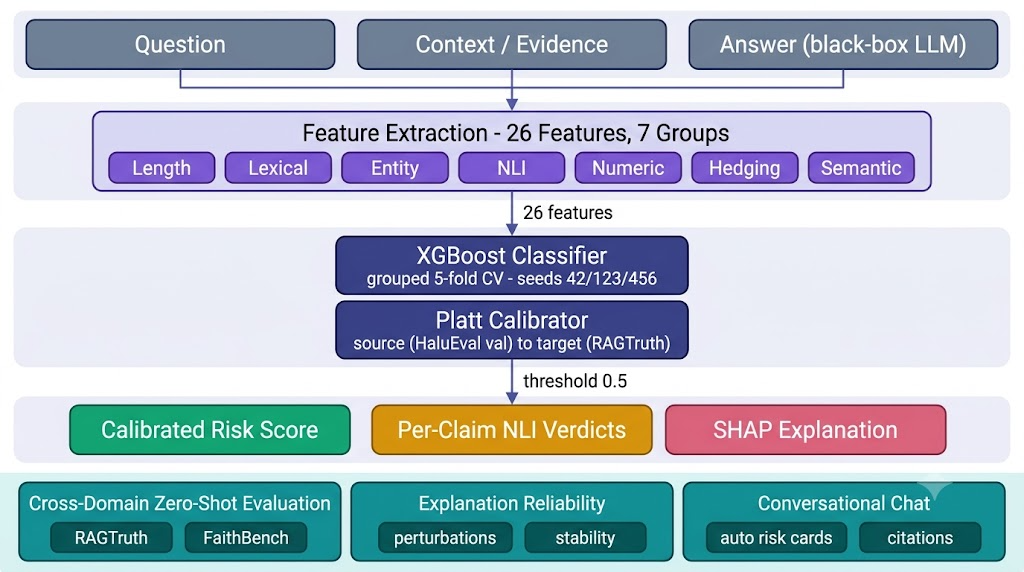
\includegraphics[width=\textwidth]{architecture.png}
\caption{End-to-end HaluRISC pipeline. Evidence-consistency features from the
question, context, and answer feed a grouped-CV trained, Platt-calibrated
XGBoost model. Outputs include a calibrated risk score, per-claim NLI
verdicts, and SHAP explanations, with cross-domain and explanation-reliability
evaluation.}
\label{fig:pipeline}
\end{figure}

\subsection{Task definition}

Given a question $q$, an optional reference context $c$ (evidence), and a candidate answer $a$ produced by a black-box LLM, the task is to predict the probability $P(\text{hallucinated} \mid q, c, a)$. HaluRISC predicts risk, not truth. It flags answers that are unsupported by, or contradictory to, the available evidence.

\subsection{Dataset and preprocessing}

The QA subset of HaluEval \cite{haluEval} provides 10{,}000 questions, each with a knowledge passage, a correct answer, and a hallucinated answer. Every question yields two rows, one per answer variant, for a total of 20{,}000 rows with perfectly balanced labels. The data is split 70/15/15 stratified by label, and the split is performed at the question-group level so that the two rows of one question never land in different splits. This grouped, leakage-free design matters because both answer variants of a question share the same context, and a random split could otherwise let the model memorize the pairing. The split indices are saved to disk for exact reproducibility.

Text is whitespace-normalized. Lexical features operate on lowercased token sets, while NER and NLI keep the original casing. Missing context is handled explicitly, with lexical overlap set to zero and NLI probabilities to one third.

\subsection{Features}

Table~\ref{tab:features} lists the 26 features in seven groups. NLI signals come from a DeBERTa-v3 cross-encoder trained on SNLI and MultiNLI, evaluated in both directions, context-to-answer and answer-to-context, which yields six probability features. Semantic similarity uses MiniLM sentence embeddings \cite{sbert}, entity features use spaCy NER, and the numeric and hedging groups are collected with regular expressions and a small hedging lexicon.

\begin{table}[t]
\centering
\small
\caption{Feature groups (26 features total).}
\label{tab:features}
\begin{tabular}{@{}lll@{}}
\toprule
\textbf{Group} & \textbf{Features} & \textbf{Source} \\
\midrule
Length/style  & n\_chars, n\_words, n\_sentences, avg\_word\_len & regex \\
Lexical       & overlap vs.\ context \& question, Jaccard $\times$2 & token sets \\
Entity        & entity counts, overlap ratio, novel-entity ratio & spaCy NER \\
NLI           & entail/contradict/neutral $\times$ 2 directions & cross-encoder NLI \\
Numeric       & number counts, overlap ratio, novel numbers & regex \\
Hedging       & hedge count, hedge density & lexicon \\
Semantic      & cosine(context,answer), cosine(question,answer) & MiniLM \\
\bottomrule
\end{tabular}
\end{table}

\subsection{Models}

Four baselines are compared. The first is a heuristic that sets risk to one minus the lexical overlap between the answer and the context, with its threshold tuned on validation. The second is logistic regression on standardized features, the third a random forest with 300 trees, and the fourth XGBoost. XGBoost hyperparameters come from a randomized search of 30 iterations over depth, learning rate, tree count, subsample, and column subsampling, scored with 5-fold stratified cross-validation on the training split. The best configuration is depth 4, learning rate 0.01, 500 trees, subsample 0.9, and column subsampling 0.7, with a cross-validated AUROC of 0.9970. Every experiment is repeated with seeds 42, 123, and 456, and results are reported as the mean over seeds.

\subsection{Calibration}

Calibrators are fit on the validation split only. Platt scaling fits a sigmoid to the raw scores, and isotonic regression fits a step function, and both are compared against the raw model on the test split with expected calibration error (10 bins), Brier score, and reliability diagrams. A second step targets a new domain. When a small labeled sample of the target corpus is available, the calibrator is re-fit on that sample, and the effect is measured on a disjoint held-out part of the target corpus.

\subsection{Explainability}

Global interpretability comes from SHAP \cite{shap}. A TreeExplainer over the raw XGBoost model produces mean absolute SHAP importance and beeswarm summaries, and local explanations show the feature contributions behind a single verdict. Explanation reliability is measured directly in this work. Each test answer is perturbed in six ways, by replacing entities, numbers, or dates, removing supporting context, inserting irrelevant context, and shuffling clauses, and the calibrated score should stay stable under neutral perturbations and react to semantic ones. Stability is quantified with Spearman and Kendall rank correlation between the original and perturbed scores, the fraction of top-1 flips, and the top-$k$ Jaccard overlap of the SHAP feature rankings.

\input{4.experiments}
\input{5.web_application}
\input{6.results_discussion}
% Chapter 7 — Conclusion and Future Work.
\section{Conclusion and Future Work}

We presented HaluRISC, a lightweight, calibrated, and explainable hallucination-risk predictor for black-box LLM outputs. On HaluEval QA it achieves F1 0.9886 with ECE 0.0051 after isotonic calibration, ~137\,ms per analysis, near-zero cost, and beats an LLM-as-judge baseline significantly at 1/100th of its cost. Its honest negative results---Platt no-gain, entity features unhelpful, RAGTruth zero-shot failure---are reported rather than hidden.

Future work (an extended study) will add cross-domain evaluation on FaithBench \cite{faithbench}, multicalibration under distribution shift, explanation-reliability metrics (feature-ablation correlation and perturbation stability), and neural baselines, targeting a Q2 applied journal.

\input{8.reproducibility}
% Chapter 9 — Ethical Considerations.
\section{Ethical Considerations}

A hallucination-risk score predicts \emph{risk}, not truth, and must not be treated as a fact-checker. Over-reliance on automated detectors creates false trust, especially when scores are confidently wrong out-of-domain (as our RAGTruth result shows). Detection quality may vary across domains and languages, and the current system is English-only. The interface therefore labels scores as risk estimates and displays a training-data warning with every prediction.


\bibliographystyle{plain}
\bibliography{ref}

\end{document}
